\chapter{Architecture of Fog VDN}
\label{chap:chap-three}
\begin{figure}[htbp]
\centering
	  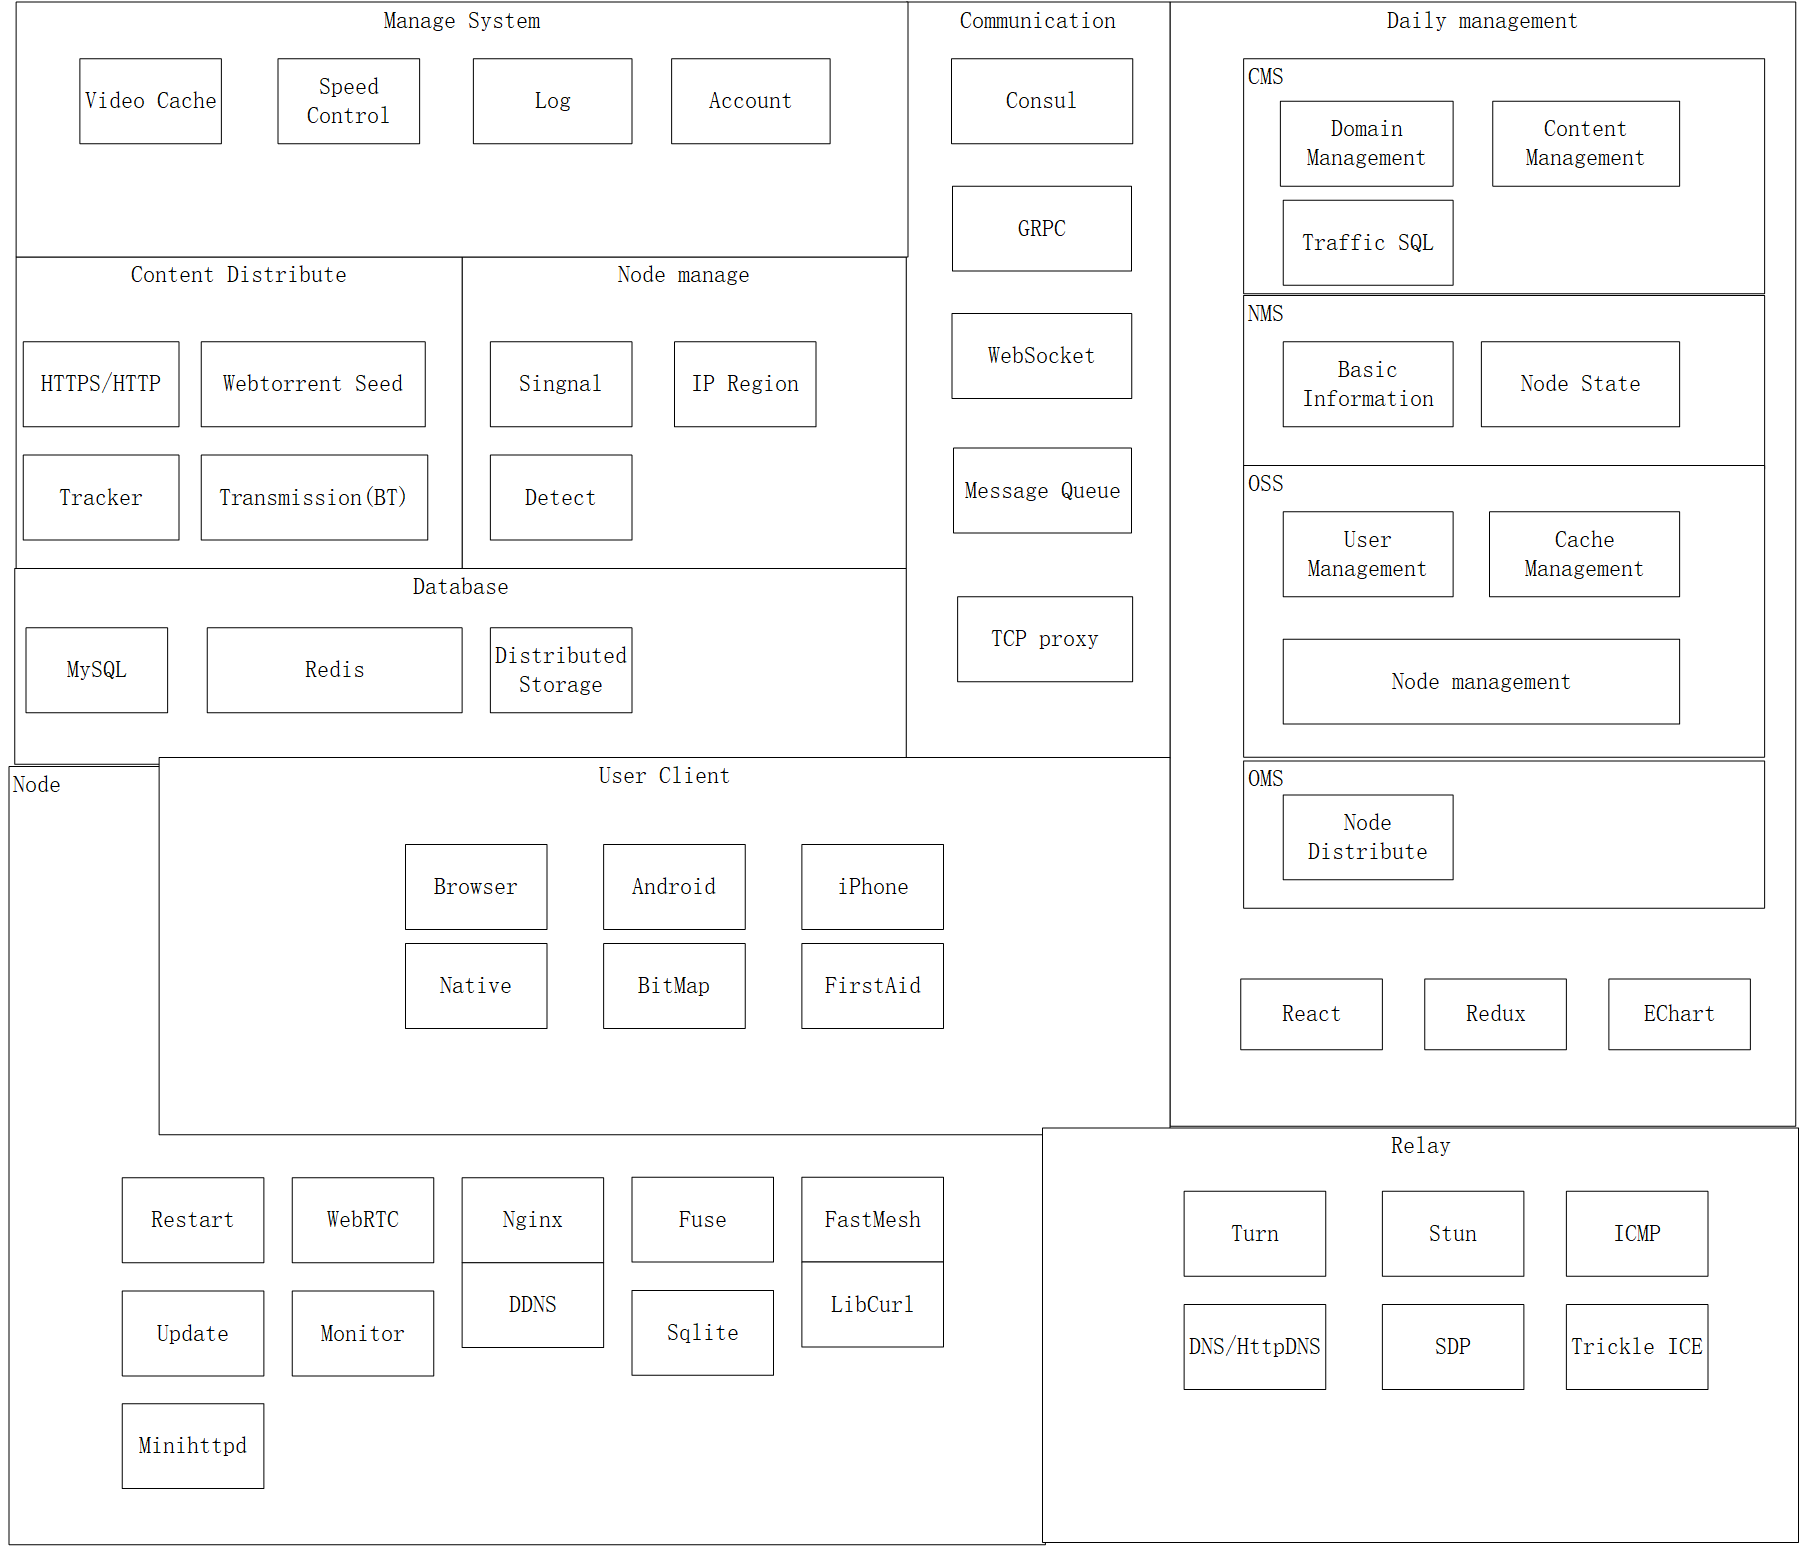
\includegraphics[width=\textwidth]{fig_6.png}
    \caption{Architecture of the Fog VDN}
	  \vskip 1.0cm
 \label{fig_6}
\end{figure}



Fog VDN is very simple(Figure \ref{fig_26}). The fog composed of the fog device
(such as Wi-Fi routers,Network Attached Storage,Smart home center,etc.) collect the
resources (bandwidth,storage,computing) combining cloud server to serve application X
(Fog as a Service FaaS,Figure \ref{fig_27}). But Fog VDN is also complex (Figure \ref{fig_6}),
composed by many systems. Whether simple or complex, Fog VDN has three subsystems,
Node System, Operations Managment System and Network Protocols.

\begin{figure}[htbp]
\centering
	  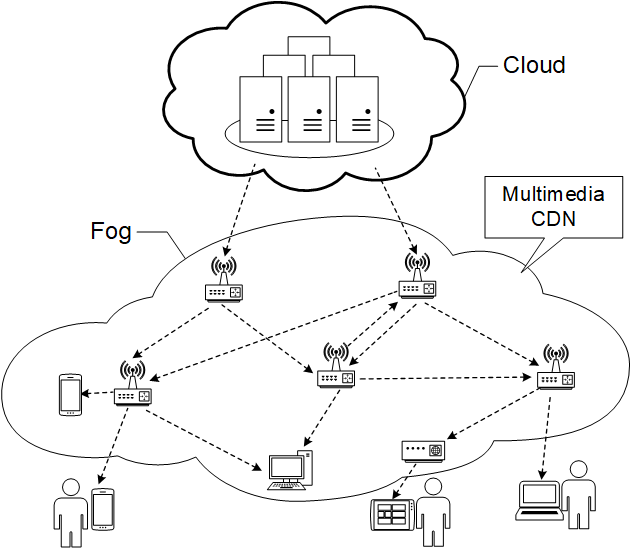
\includegraphics[width=0.8\textwidth]{fig_26.png}
    \caption{Simple architecture of the Fog VDN}
 \label{fig_26}
\end{figure}

\section{Node System}

\begin{figure}[htbp]
\centering
	  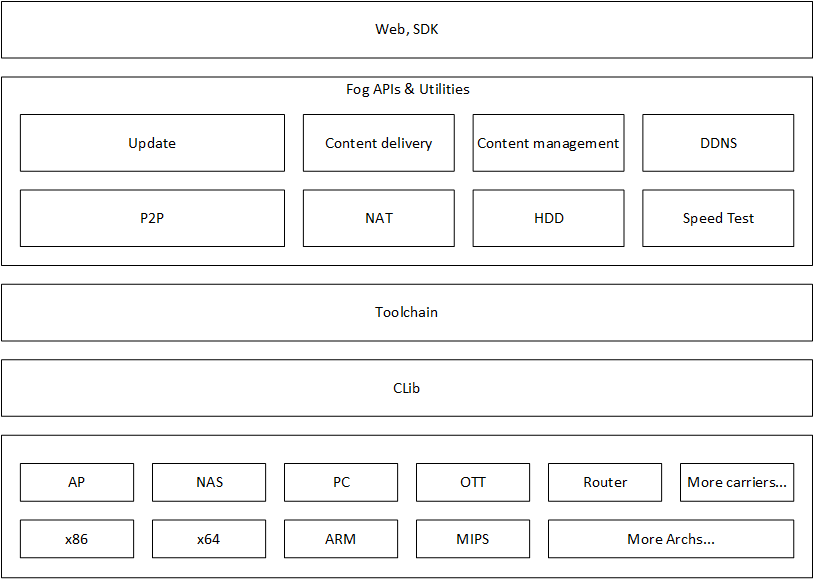
\includegraphics[width=\textwidth]{fig_25.png}
    \caption{ Architecture of the Fog nodes}
 \label{fig_6}
\end{figure}

  \subsection{Fog devices}
    \label{Fog devices}
  There are many different types about fog nodes, "Personal Computer"(PC), "Network Attached Storage"(NAS),
WirelessAccessPoint,Router,Mobile,Base Station all included. In this thesis, we only talk about the fog nodes
which can run the Fog VDN well, which generally have a large storage(>16GB), ROM(>32MB) and RAM(>512MB).
  For hardware devices, there are too many different platforms and configurations to easily unified.
Different from Xunlei and Youku product same hardware, also not same as Huawei use a heavy JVM platform,
 We use the C programing in order to minimize the size of program, so that it can run well in the fog
nodes and we can code once, compile everywhere.
 \subsection{Basic module}

  \begin{itemize}
    \item Node\_update  : update the program in node.
    \item Node\_restart : restart if the process broken down.
    \item Node\_monitor : monitor the process.
    \item Node\_report  : report the node basic information every 5 minutes.
    \item Node\_p2p     : connect to the other fog node.
    \item Node\_log     : record the node run time information.
    \item Node\_file    : manage the data in the nodes.
  \end{itemize}

  Fig \ref{fig_36} shows the relationship between these basic module.
 \subsection{General fog node}
 One of the most famous design philosophy of peer-to-peer system is sharing. As an application of P2P,
we also inherit the spirit of sharing. A special fog node  means the nodes which we refer to in section
\ref{Fog devices} . A general fog node include not only special fog node, but also the client. Figure
\ref{fig_34} is a fog player client, the red block is downloaded from the cloud, the blue, yellow and green
block is downloaded from special fog node. The purple block is downloaded from the client who is watching
this video. This is general fog node, same as conventional P2P node.

\begin{figure}[htbp]
\centering
	  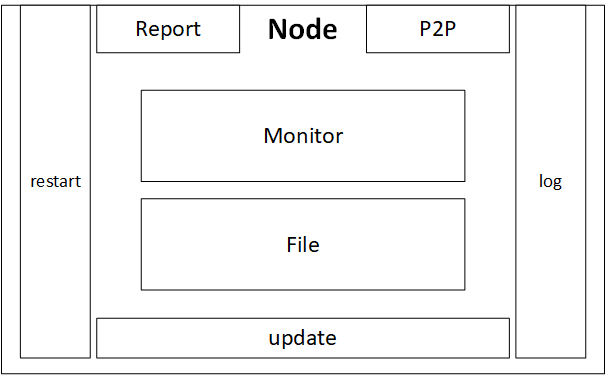
\includegraphics[width=0.8\textwidth]{fig_36.png}
    \caption{ Architecture of the Fog nodes System.}
 \label{fig_36}
\end{figure}

\section{Operations Managment System}



\begin{figure}[htbp]
\centering
	  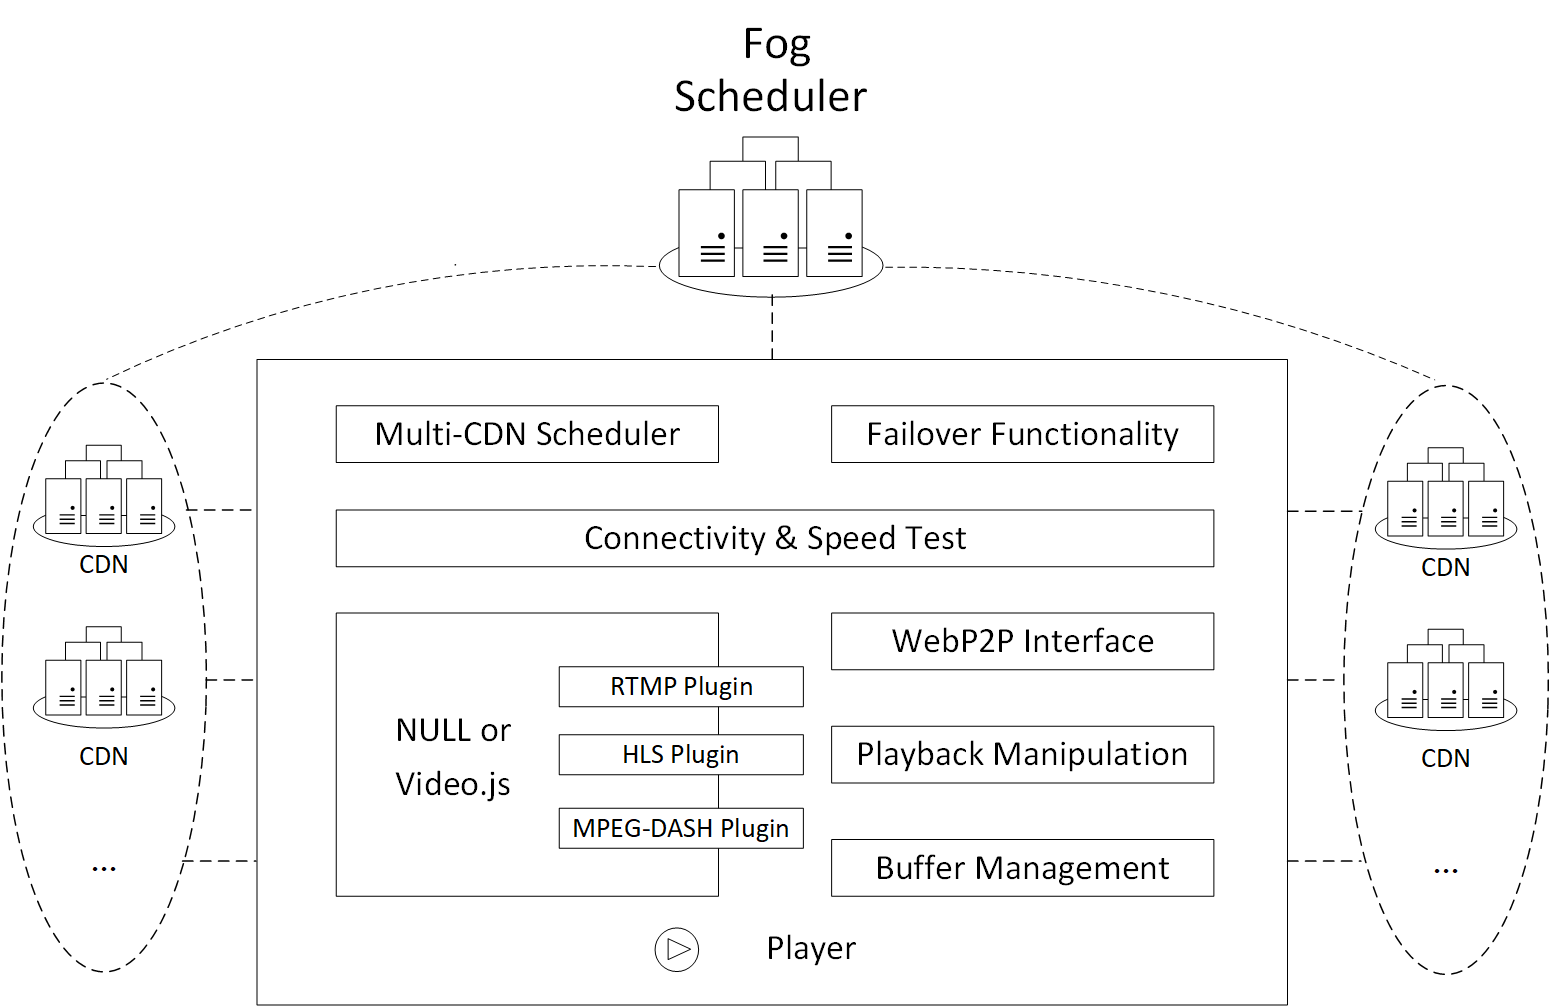
\includegraphics[width=\textwidth]{fig_7.png}
    \caption{Architecture of the Fog Player}
	  \vskip 1.0cm
 \label{fig_7}
\end{figure}

\begin{figure}[htbp]
\centering
	  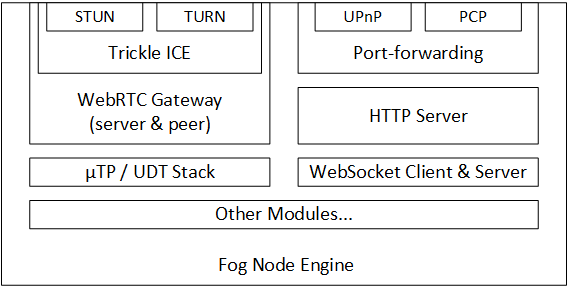
\includegraphics[width=\textwidth]{fig_8.png}
    \caption{Architecture of the Fog Node Engine}
 \label{fig_8}
\end{figure}

\begin{figure}[htbp]
\centering
	  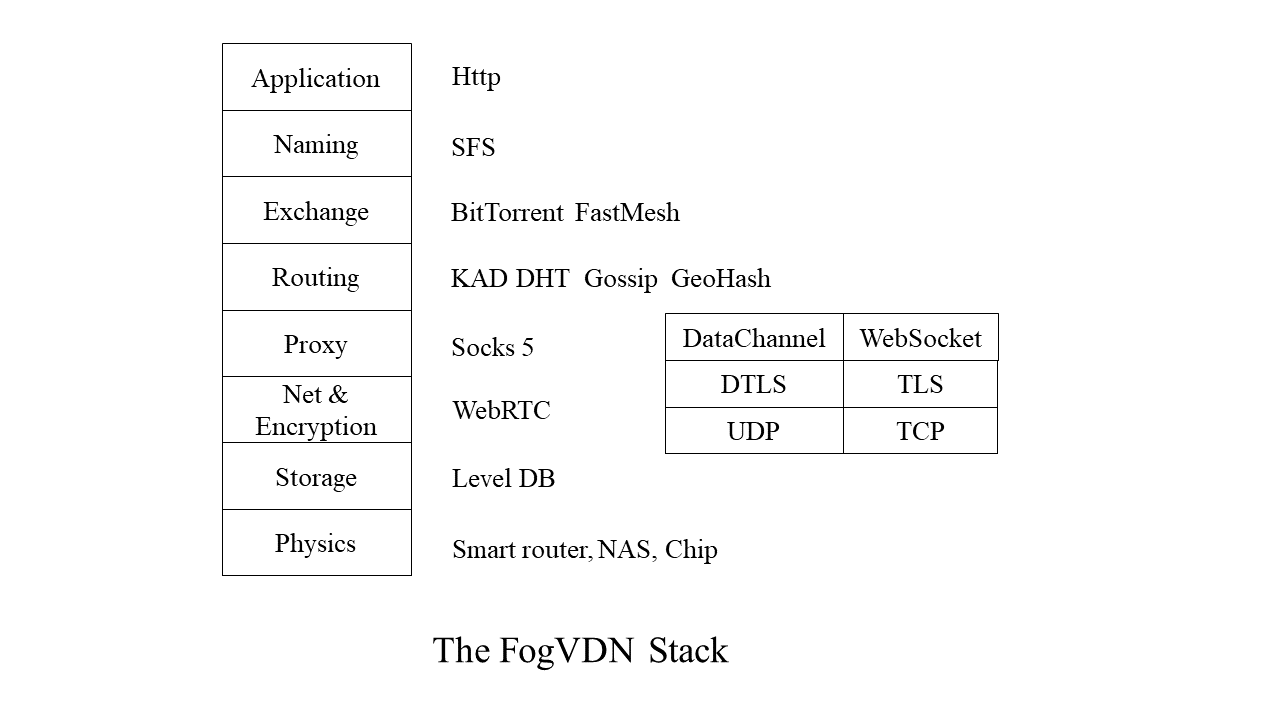
\includegraphics[width=\textwidth]{fig_17.png}
    \caption{Fog VDN Stack}
 \label{fig_17}
\end{figure}
